\documentclass[11pt, a4paper]{article}

% --- Packages ---
\usepackage[utf8]{inputenc}
\usepackage[T1]{fontenc}
\usepackage[margin=1in]{geometry}
\usepackage{amsmath, amssymb}
\usepackage{graphicx}
\usepackage{hyperref}
\usepackage{listings}
\usepackage{xcolor}
\usepackage{booktabs}
\usepackage{float}
\usepackage{enumitem}
\usepackage{abstract}
\usepackage{tikz}
\usetikzlibrary{arrows.meta, positioning, shapes.geometric, decorations.pathreplacing}

% --- Hyperlink styling ---
\hypersetup{
    colorlinks=true,
    linkcolor=blue!70!black,
    citecolor=blue!70!black,
    urlcolor=blue!70!black
}

% --- Code listing style ---
\definecolor{codebg}{RGB}{245,245,245}
\definecolor{codegreen}{RGB}{0,128,0}
\definecolor{codegray}{RGB}{128,128,128}
\definecolor{codeblue}{RGB}{0,0,180}

\lstset{
    backgroundcolor=\color{codebg},
    basicstyle=\ttfamily\small,
    breaklines=true,
    captionpos=b,
    commentstyle=\color{codegreen},
    keywordstyle=\color{codeblue}\bfseries,
    stringstyle=\color{red!70!black},
    numberstyle=\tiny\color{codegray},
    numbers=left,
    numbersep=8pt,
    frame=single,
    framerule=0.5pt,
    rulecolor=\color{gray!50},
    tabsize=4,
    showstringspaces=false
}

% --- Title ---
\title{\textbf{Quantum-Safe Bitcoin Transactions Today}}
\author{Avihu Mordechai Levy\footnote{\texttt{avihu@starkware.co}, socials: \texttt{@avihu28}}\\StarkWare}
\date{\today}

\begin{document}

\maketitle

\begin{abstract}
We present the first quantum-safe Bitcoin transaction scheme that requires no changes to the Bitcoin protocol and remains secure even in the presence of Shor's algorithm. Our construction modifies \textsc{Binohash} (Linus, 2026), replacing its non-quantum-safe component---the signature-size-based proof-of-work puzzle---with a hash-to-sig puzzle whose security depends only on the pre-image resistance of RIPEMD-160. The resulting scheme, Quantum Safe Bitcoin (QSB), achieves ${\sim}118$-bit second pre-image resistance under the Shor threat model (roughly half under Grover's algorithm), at an estimated off-chain GPU cost of a few hundred dollars. The scheme fits within Bitcoin's legacy script constraints of 201 opcodes and 10{,}000 bytes.
\end{abstract}

% ============================================================
\section{Introduction}
\label{sec:introduction}
% ============================================================

Bitcoin transactions are not quantum-safe. The primitive that binds the components of a transaction---its inputs, outputs, and spending conditions---is an ECDSA signature (pre-Taproot) or a Schnorr signature (post-Taproot), neither of which is post-quantum secure. This means that even spending conditions which are themselves quantum-safe can be subverted: if the signature scheme securing the transaction is broken, the entire transaction---including its outputs and other inputs---can be forged.

Consider, for example, a UTXO whose spending condition is knowledge of a hash preimage, which is quantum-safe on its own. A spender broadcasts a transaction revealing the preimage. An adversary who can break the signature scheme can take that preimage, construct a different transaction~$t'$ spending the same UTXO to an address they control, sign~$t'$ with a forged signature, and broadcast it instead.\footnote{Under Taproot, the situation is strictly worse: every Taproot output is spendable via the key path, meaning knowledge of the private key corresponding to the internal public key (which aggregates the taptweak and the script tree root) suffices to spend it, regardless of the script conditions in the taptree~\cite{bip341}. A quantum adversary capable of computing discrete logarithms could therefore spend any Taproot output directly.}

% ============================================================
\subsection{Related Work}
\label{sec:related-work}
% ============================================================

Two recent works bring us close to the goal of quantum-safe Bitcoin transactions. The first is Heilman's ``Signing a Bitcoin Transaction with Lamport Signatures (no OP\_CAT)''~\cite{heilman2024}, followed by the work of Robin Linus---\textsc{Binohash}~\cite{linus2024binohash}---on which the present scheme is based.

While these two works differ significantly in their constructions and security properties, they both rely on a common high-level approach. Inside the Script:

\begin{enumerate}
    \item \textbf{Derive a cryptographically strong identifier} of the spending transaction---call it~$D$.
    \item \textbf{Verify a Lamport signature} over~$D$.
\end{enumerate}

Since Lamport signatures are post-quantum secure, and they sign a cryptographically strong identifier of the transaction, it is not possible to modify the transaction without producing a new Lamport signature---which the attacker cannot forge, even with quantum computing capabilities.

\subsubsection{Remaining Issues}
\label{sec:issues}

There are two main issues with the existing schemes:

\paragraph{1. Reliance on signature size check.}
This is the central issue. Both schemes rely on a signature proof-of-work (PoW) puzzle based on signature size~\cite{borco2024}, verified via \texttt{OP\_SIZE}. This puzzle assumes a specifically small ECDSA $r$ value for which the discrete logarithm is known. Currently, a well-known minimal value~$r_{\min}$ is used. However, an adversary with knowledge of discrete logarithms---as a quantum computer would provide---could compute the smallest possible $r$ value ($r = 1$), breaking the \texttt{OP\_SIZE} check for all transactions created with the current~$r_{\min}$.\footnote{Paradoxically, once $r = 1$ is found, it could be used \emph{going forward} to strengthen these schemes: the PoW puzzle with $r = 1$ would be quantum-safe, since there is no smaller $r$ to exploit. But all transactions created before that point, using the current~$r_{\min}$, would be vulnerable.}

\paragraph{2. Sighash flag uncertainty.}
Since the sighash flag is not directly readable from Script, both works acknowledge potential attacks arising from this limitation. \textsc{Binohash} discusses this in detail~\cite[Section~7.1]{linus2024binohash}, identifying \texttt{ANYONECANPAY|NONE} as a potential attack vector that could break the security guarantees.

\subsection{Our Contribution}
\label{sec:contribution}

In this work, we modify the \textsc{Binohash} scheme to address both issues identified in Section~1.1.1. We replace the signature-size-based PoW puzzle with a hash-to-sig puzzle: the script hashes a transaction-bound public key via RIPEMD-160 and checks whether the output is a valid DER signature---an event with probability~${\sim}2^{-46}$, independent of any elliptic curve hardness assumption. Since the puzzle's signature is hardcoded with \texttt{SIGHASH\_ALL}, the sighash flag uncertainty is also eliminated.

We further introduce \emph{bonus keys}---subset selections that contribute to the search space without requiring HORS verification---to bridge the gap between the fixed $2^{46}$ puzzle target and the available opcode budget. The resulting scheme achieves~${\sim}118$-bit pre-image resistance and fits within 201 opcodes, at an off-chain GPU cost of a few hundred dollars.

\subsection{Discussion}

While this article describes a solution that is practical, affordable, and works today for quantum-safe Bitcoin transactions, it should be treated as a last-resort measure. This is because both the off-chain computational cost and the on-chain transaction cost do not scale to the full range of users, amounts, and throughput that Bitcoin targets. To the extent that the quantum threat is believed to be real, it remains necessary to continue the ongoing effort to research and implement the best possible solution for Bitcoin---one that is user-friendly, maximally efficient, and secure by design, ideally through protocol-level changes.

% ============================================================
\section{Background}
\label{sec:background}
% ============================================================

We assume familiarity with Bitcoin Script, ECDSA signatures, and DER encoding; for a thorough treatment of these topics, see \textsc{Binohash}~\cite{linus2024binohash}, Sections~2--3. Our scheme builds extensively on the \textsc{Binohash} construction, and we strongly recommend reading that paper prior to this one. While we summarize the relevant components in the following sections, many of the deeper design choices and optimizations---particularly around FindAndDelete, minimum-size signatures, and the SIGHASH\_SINGLE bug---are explained more fully there.

\subsection{Goals}
\label{sec:goals}

We aim to construct:
\begin{enumerate}
    \item A \textbf{cryptographically strong identifier} of the spending transaction---with both second pre-image and collision resistance---that is readable within Bitcoin Script.
    \item A \textbf{Lamport signature} over that identifier, verifiable entirely within Script.
\end{enumerate}

\subsection{Constraints}
\label{sec:constraints}

For multiple reasons---including the reliance on ECDSA (rather than Schnorr), the FindAndDelete mechanism (removed in SegWit), and the SIGHASH\_SINGLE bug (absent in SegWit's sighash algorithm)---neither \textsc{Binohash} nor our construction can use Taproot or SegWit. We are therefore restricted to legacy (pre-SegWit) script execution, which imposes severe constraints. The two hardest, and therefore most important, are:

\begin{enumerate}
    \item \textbf{Opcode limit.} The number of non-push opcodes in a script may not exceed 201. Every opcode above \texttt{OP\_16} counts toward this limit, including opcodes in non-executed branches of \texttt{OP\_IF}/\texttt{OP\_ELSE}~\cite[Section~6]{linus2024binohash}.
    \item \textbf{Script size limit.} The total script size may not exceed 10,000 bytes~\cite[Section~6]{linus2024binohash}.
\end{enumerate}

\noindent For a full discussion of additional constraints---including stack element size limits, stack depth, and transaction relay considerations---see \textsc{Binohash}~\cite[Section~6]{linus2024binohash}.

These constraints are extremely demanding in the context of our two goals: achieving a cryptographically strong transaction identifier requires a high number of security bits, while the Lamport signature imposes a per-bit overhead in both opcodes and script size.

\subsection{Threat Model}
\label{sec:threat-model}

\subsubsection{Quantum Computing Assumptions}
\label{sec:quantum-assumptions}

Our threat model assumes an adversary with access to a cryptographically relevant quantum computer. We distinguish between the two classes of cryptographic primitives affected:

\paragraph{Elliptic curve cryptography (catastrophic vulnerability).}
ECDSA and Schnorr signatures rely on the hardness of the elliptic curve discrete logarithm problem (ECDLP). Shor's algorithm~\cite{shor1994} solves ECDLP in polynomial time on a quantum computer, rendering these schemes completely insecure. For the secp256k1 curve used in Bitcoin, a sufficiently large quantum computer could recover private keys from public keys, forge arbitrary signatures, and compute discrete logarithms of any curve point. This is a total break: the adversary gains \emph{unlimited} forgery capability, not merely a reduction in work factor.

\paragraph{Hash functions (moderate weakening).}
Cryptographic hash functions such as SHA-256, RIPEMD-160, and HASH160 are affected by Grover's algorithm~\cite{grover1996}, which provides a quadratic speedup for unstructured search. This reduces the effective security of an $n$-bit hash from~$2^n$ to~$2^{n/2}$ for pre-image attacks, and from~$2^{n/2}$ to~$2^{n/3}$ for collision attacks. Importantly, this is a \emph{weakening}, not a break: a 160-bit hash retains approximately 80 bits of pre-image resistance and approximately 53 bits of collision resistance against a quantum adversary. For our scheme, which relies on RIPEMD-160 (160 bits), this provides a comfortable security margin.

\paragraph{Practical timeline considerations.}
While the timeline for large-scale fault-tolerant quantum computers remains uncertain, there is broad consensus that breaking elliptic curve cryptography is likely to be feasible significantly earlier than breaking hash functions to a practically exploitable degree. Shor's algorithm requires a number of logical qubits roughly proportional to the key size, while Grover's algorithm---though polynomial in qubits---offers only a quadratic speedup and is difficult to parallelize. This asymmetry motivates our approach: we aim to eliminate \emph{all} reliance on elliptic curve hardness for security, while retaining hash-based primitives whose quantum-reduced security levels remain adequate.

\subsubsection{Security Requirements}

In the context of quantum-safe transactions, there are two distinct security properties we aim to achieve. They differ significantly in severity and in the assumptions they make about the adversary.

\paragraph{1. Second pre-image resistance (critical).}
This is the primary security requirement. Suppose an honest spender broadcasts a transaction~$T$ whose digest is~$D = H(T)$. We require that it is infeasible for a malicious actor---even one equipped with a quantum computer---who observes~$T$ and its digest~$D$ to construct a different transaction~$T'$ such that~$H(T') = D$. If such a~$T'$ could be found, the attacker could reuse the Lamport signature revealed in~$T$ to authorize~$T'$, completely breaking the quantum safety of the scheme.

\paragraph{2. Collision resistance (secondary).}
Here we consider a potentially malicious spender who controls the transaction creation process. We require that the spender cannot find two distinct transactions~$T$ and~$T'$ such that~$H(T) = H(T')$. This property is not essential for the spender's own quantum safety---the spender has no incentive to attack their own transaction---but it prevents equivocation: the spender cannot present one transaction to a counterparty while secretly holding another, equally valid transaction with a different set of outputs. This is particularly relevant for protocols such as BitVM~\cite{linus2024binohash} that rely on the uniqueness of the digest for off-chain dispute resolution.

\subsection{Binohash Overview}
\label{sec:binohash-overview}

\noindent\textit{Readers already familiar with \textsc{Binohash}~\cite{linus2024binohash} may skip to Section~\ref{sec:scheme}, where we present our modifications.}

\medskip

At a high level, to create a valid spending transaction with \textsc{Binohash}, the spender must complete two steps of proof-of-work:

\paragraph{Step 1: Transaction pinning.}
Force a~$W_1$-bit PoW puzzle for every change to the spending transaction. This means the spender must perform~$2^{W_1}$ additional work each time any part of the transaction is modified.

\paragraph{Step 2: Compute the Binohash digest.}
Find a valid hash digest~$D$ for the transaction. A valid digest is constructed from two rounds of ``$n$-choose-$t$'' subset selections over signatures embedded in the script---hence the name \textsc{Binohash}. The correct combination of signatures results in solving an additional~$W_2$-bit PoW puzzle per round. The selected subsets form the digest~$D$, which is also Lamport-signed within the script.

The Lamport signature uses a HORS (Hash to Obtain Random Subset) scheme~\cite{reyzin2002}: for each of the~$n$ possible indices, the locking script contains a hash commitment~$H(\mathit{pre}_i)$. To sign a particular subset (the digest), the spender reveals the preimages~$\mathit{pre}_i$ for the selected indices. The script verifies each preimage by hashing it and comparing to the commitment. Since preimages are secret until revealed, the spender commits to a specific digest at signing time.

\medskip

The total work for the honest spender is therefore~$2^{W_1} + 2 \cdot 2^{W_2}$. The digest~$D$ has~$2 W_2$ bits of entropy.

\paragraph{Second pre-image resistance.}
Both steps contribute equally to this property. Given a transaction~$T$ with~$H(T) = D$, finding a different transaction~$T'$ with~$H(T') = D$ costs~$2^{W_1}$ per attempt (due to pinning), and the expected number of attempts to match~$D$ is~$2^{2 W_2}$ (the digest space). The total cost is~$2^{W_1} \cdot 2^{2 W_2}$.

\paragraph{Collision resistance and the role of pinning.}
The value of Step~1 (pinning) becomes apparent when we consider collision resistance. Due to the birthday attack, finding two transactions with the same digest costs only~$2^{W_2}$ samples (the square root of the~$2^{2W_2}$ digest space). However, generating each sample still requires~$2^{W_1}$ work for pinning. The total collision cost is therefore~$2^{W_1 + W_2}$, and the~$W_1$ contribution from pinning is the dominant factor.

Additionally, pinning is extremely cheap in terms of both opcodes and script size, while still providing valuable security. Why not increase~$W_1$ further? Because the pinning cost is imposed on the honest spender as well. The optimal strategy is to set~$W_1$ roughly equal to the work the spender already performs to find the digest, which is approximately~$2 \cdot 2^{W_2}$. This balances the cost borne by the spender against the security gained.

\subsection{Why a Binomial Structure?}
\label{sec:binomial-intuition}

The opcode constraint is extremely severe. Achieving a target security of ${\sim}100$ bits---with a digest that is also Lamport-signed---within a budget of 201 non-push opcodes is a formidable challenge.

The digest information must be provided by the unlocking script (the witness). If it were supplied as many independent elements, the cost of processing and signing each one would be prohibitive. Conversely, reproducing many elements in the locking script from a few witness-provided values is equally expensive: flow-control opcodes (\texttt{OP\_IF}/\texttt{OP\_ELSE}) count toward the 201-opcode limit even in non-executed branches, making dispatch logic impractical.

We are therefore forced to encode the digest in a \emph{small number of witness elements}, and to verify and sign it with correspondingly few operations. This naturally leads to a binomial structure: the witness provides $t$ indices selecting a subset from a pool of~$n$ items embedded in the locking script. The number of possible subsets, $\binom{n}{t}$, grows rapidly even for small~$t$, providing the entropy we need. For example, $\binom{150}{8} \approx 2^{42}$ with just 8 selections.

\subsection{Primitives}
\label{sec:primitives}

To perform proof of work over a transaction that is checkable in Script, we need two ingredients:

\begin{enumerate}
    \item \textbf{A method to verify PoW in Script.} Given a candidate solution, the script must be able to check that sufficient work was performed. This is the role of the \emph{signature size puzzle} (Section~\ref{sec:sig-size-puzzle}).

    \item \textbf{A method to iterate over candidates.} The spender must be able to try many candidates until one satisfies the PoW check. This iteration itself splits into two distinct mechanisms:

    \begin{enumerate}
        \item \textbf{Iteration outside the script.} The spender modifies transaction parameters---such as \texttt{nLocktime}, output ordering, or \texttt{OP\_RETURN} data---and re-checks the PoW puzzle in Script for each variant. Since these modifications happen outside the script, they are \emph{not} Lamport-signable. This is essentially what is used for \emph{transaction pinning} (Step~1): the spender iterates over transaction variants off-chain, and the script verifies the PoW for whichever variant is broadcast.

        \item \textbf{Iteration inside the script.} Here, different iterations are invoked by different data provided in the unlocking script (witness). Crucially, this data \emph{is} Lamport-signable within the script, which is what makes it suitable for the digest (Step~2). For this to be practical, we need an efficient method to iterate over many candidates with as few opcodes and bytes as possible. This is the role of the \emph{FindAndDelete mechanism} (Section~\ref{sec:findanddelete}).
    \end{enumerate}
\end{enumerate}

\subsubsection{Signature Size Puzzle}
\label{sec:sig-size-puzzle}

The signature size puzzle, introduced by Bor~\cite{borco2024} and refined by Linus~\cite{linus2024binohash}, exploits the fact that a DER-encoded ECDSA signature's total byte length is determined by the lengths of its two components, $r$ and~$s$. If~$r$ is fixed, then the total signature size is governed solely by the length of~$s$, and finding an~$s$ shorter than a target threshold requires brute-force search---a proof of work. The way to effectively fix~$r$ is by imposing an extreme constraint on the total signature size, practically forcing the spender to use the smallest known~$r$ value; any larger~$r$ would make it infeasible to meet the size target.

Concretely, the puzzle works as follows:

\begin{enumerate}
    \item \textbf{Force a fixed~$r$ via size constraint.} The locking script enforces a signature size threshold so tight that only signatures using the smallest known~$r$ value---$r_{\min}$, whose $x$-coordinate is approximately 21 bytes---can satisfy it. The discrete logarithm of the corresponding curve point is known, allowing anyone to compute signatures with this specific~$r$.

    \item \textbf{Grind for small~$s$.} To solve the puzzle, the spender searches over transactions (or nonces) until the resulting ECDSA signature---computed with the known~$r_{\min}$---has an~$s$ value short enough that the total DER-encoded signature falls below the target size.

    \item \textbf{Verify via \texttt{OP\_SIZE}.} Bitcoin Script cannot parse the internal structure of a signature, but it can measure its total byte length using \texttt{OP\_SIZE}. By checking that the signature is shorter than a threshold, the script implicitly verifies that sufficient grinding was performed.
\end{enumerate}

This primitive is elegant and cheap: verification requires only \texttt{OP\_SIZE} and an \texttt{OP\_LESSTHAN} or \texttt{OP\_EQUALVERIFY}---just 2--3 opcodes.

\subsubsection{FindAndDelete and Sighash Variation}
\label{sec:findanddelete}

The signature size puzzle gives us a way to verify proof of work on a single signature. But for Step~2---computing the digest---we need to iterate over many candidates \emph{inside} the script, in a way that is Lamport-signable. The mechanism that makes this possible is \emph{FindAndDelete}---a legacy quirk of how \texttt{OP\_CHECKMULTISIG} computes sighashes in pre-SegWit Bitcoin.

When \texttt{OP\_CHECKMULTISIG} verifies a signature, it first computes the sighash---the double-SHA256 of the transaction data that the signature commits to. Crucially, the sighash is computed over the \emph{scriptCode}, which is the locking script with all signature data removed via a process called FindAndDelete: before hashing, the script interpreter scans the scriptCode and deletes every occurrence of each signature being verified.

\textsc{Binohash} exploits this as follows. The locking script embeds~$n$ dummy signatures (e.g., $n = 150$). The spender selects a subset of~$t$ of them and passes them to \texttt{OP\_CHECKMULTISIG}. FindAndDelete removes exactly those~$t$ signatures from the scriptCode before computing the sighash. A different subset of~$t$ signatures leads to a different scriptCode, and therefore a different sighash.

This gives the spender $\binom{n}{t}$ distinct sighashes to try---all from a single, fixed transaction. For each sighash, the spender checks whether the corresponding PoW puzzle is satisfied. The subset that solves the puzzle becomes the digest.

The dummy signatures are constructed to be transaction-independent using the \texttt{SIGHASH\_SINGLE} bug: when \texttt{SIGHASH\_SINGLE} is used for an input whose index exceeds the number of outputs, Bitcoin sets the signed message to~$z = 1$, regardless of the transaction content~\cite{linus2024binohash}. This allows the dummy signatures and their corresponding public keys (recovered via ECDSA key recovery with $z = 1$) to be precomputed once and reused across all transactions.

\noindent FindAndDelete was removed in SegWit (BIP~143~\cite{bip143}), which is one of the reasons this construction requires legacy (pre-SegWit) script execution.

\subsection{The Binohash Scheme}
\label{sec:binohash-scheme}

We now describe how the primitives above are assembled into the full \textsc{Binohash} construction. For a complete treatment, see~\cite{linus2024binohash}.

\subsubsection{Script Verification (Locking Script)}

\paragraph{Step 1: Transaction pinning.}
The locking script verifies four signature size puzzles, each using a different sighash flag combination, to cover all possible transaction modification vectors.\footnote{Since Bitcoin Script cannot enforce which sighash flag the spender uses, the spender could choose any of the six available modes. Two of these are \texttt{SIGHASH\_SINGLE} variants, which are eliminated by an explicit check that detects the $z = 1$ bug. The remaining four modes---\texttt{ALL}, \texttt{NONE}, \texttt{ALL|ANYONECANPAY}, and \texttt{NONE|ANYONECANPAY}---are each assigned a separate puzzle. By requiring all four puzzles to be solved, we ensure that regardless of which mode the spender uses, every transaction field is committed to by at least one puzzle. See~\cite[Section~5]{linus2024binohash} for details.} The four distinct puzzles can be enforced either via \texttt{OP\_CODESEPARATOR}---which changes the scriptCode used for sighash computation at each invocation---or via a more compact trick involving carefully chosen public keys; see~\cite[Appendix~A]{linus2024binohash}. Additionally, the \texttt{SIGHASH\_SINGLE} flag is explicitly excluded via a check, preventing an attacker from using the $z = 1$ bug to bypass the PoW. This step costs 13 opcodes.

\paragraph{Step 2: Digest verification (two rounds).}
Each round performs the following:

\begin{enumerate}
    \item \textbf{Lamport signature verification.} The spender reveals HORS preimages for the selected subset indices. The script verifies each preimage against its corresponding hash commitment (embedded in the locking script).

    \item \textbf{Dummy signature subset selection.} Based on the indices provided in the witness, the script uses \texttt{OP\_ROLL} to select~$t$ dummy signatures from the pool of~$n$.

    \item \textbf{Multisig verification with puzzle signature.} The selected dummy signatures, together with the puzzle signature, are verified via \texttt{OP\_CHECKMULTISIG}. FindAndDelete removes the selected dummies from the scriptCode, so the puzzle signature's sighash reflects the specific subset chosen.

    \item \textbf{PoW check.} The puzzle signature's size is checked via \texttt{OP\_SIZE} against the~$W_2$ target.
\end{enumerate}

\subsubsection{Spending Procedure (Off-Chain)}

To find a valid spending transaction, the spender performs the following:

\begin{enumerate}
    \item \textbf{Solve the pinning puzzle.} Iterate over transaction parameters (e.g., \texttt{nLocktime}, output ordering) until all four pinning puzzles are satisfied. The transaction is now fixed.

    \item \textbf{Search for the digest.} For each round, iterate over the $\binom{n}{t}$ possible dummy signature subsets. Each subset produces a different scriptCode via FindAndDelete, yielding a different sighash. Check whether the resulting puzzle signature satisfies the~$W_2$-bit PoW target.

    \item \textbf{Record the digest.} The subset that solves the puzzle becomes the digest for that round. Reveal the corresponding HORS preimages (Lamport signature).

    \item \textbf{Repeat for both rounds.} If both rounds find a solution---the full digest is complete. If either round fails (none of the $\binom{n}{t}$ subsets solve the puzzle), return to step~1 with a modified transaction and try again.
\end{enumerate}

\subsection{Open Issues}
\label{sec:open-issues}

Before presenting our scheme, we identify two issues with the \textsc{Binohash} construction as described above. The first is a fundamental quantum safety vulnerability---a direct consequence of the catastrophic weakness of elliptic curve cryptography under quantum computing (Section~\ref{sec:quantum-assumptions}). The second is a sighash-related attack that, while not specific to quantum computing, must be addressed for standalone use outside of BitVM.

\subsubsection{The Signature Size Puzzle Is Not Quantum Safe}
\label{sec:quantum-vulnerability}

The signature size puzzle (Section~\ref{sec:sig-size-puzzle}) relies on the assumption that the spender is forced to use the smallest known $r$ value,~$r_{\min}$, when constructing the puzzle signature. This assumption holds classically: finding a different curve point with a comparably small $x$-coordinate requires approximately~$2^{96}$ work~\cite[Section~4]{linus2024binohash}.

As discussed in Section~\ref{sec:quantum-assumptions}, a quantum computer running Shor's algorithm~\cite{shor1994} can compute the discrete logarithm of \emph{any} elliptic curve point in polynomial time. This includes points with very small $x$-coordinates---in particular, the point with $r = 1$ (or the smallest valid $r$ on the curve). Armed with this value, the adversary can produce signatures with a shorter~$r$ than~$r_{\min}$, allowing them to satisfy the \texttt{OP\_SIZE} check with significantly less work on~$s$---or none at all.

Concretely: the PoW difficulty is determined by how short~$s$ must be to bring the total signature size under the target threshold. If the target requires~$W$ bits of grinding on~$s$ when using~$r_{\min}$, then an adversary who finds a curve point with an~$r$ value just~$\lceil W/8 \rceil$ bytes shorter than~$r_{\min}$ gains enough headroom to satisfy the size check with virtually any~$s$, reducing the PoW to zero. For typical targets of~$W \approx 40$, this means finding an~$r$ just 5 bytes shorter than~$r_{\min}$ suffices to break the puzzle entirely.\footnote{As noted in Section~1.1.1, once the discrete logarithm for the smallest valid~$r$ is known, the puzzle \emph{could} be redesigned around it. But all existing transactions created using~$r_{\min}$ would remain vulnerable.}

Note that this vulnerability is fundamentally different from the weakening of hash functions by Grover's algorithm. While Grover reduces hash security by a square root factor, the result remains computationally hard (e.g., RIPEMD-160 retains~${\sim}2^{80}$ pre-image resistance). Shor's attack on the signature size puzzle, by contrast, is a \emph{total break}: the PoW guarantee collapses entirely, regardless of the target difficulty.

\subsubsection{Sighash Flag Uncertainty}
\label{sec:sighash-vulnerability}

The second issue concerns the sighash flag byte appended to each signature. As discussed in Section~\ref{sec:binohash-scheme}, the pinning stage uses four separate puzzles to cover all non-\texttt{SINGLE} sighash modes. However, this protection applies only to the pinning signatures.

The puzzle signatures in Step~2 (the digest rounds) are produced by the spender via PoW grinding. The spender is free to choose any sighash flag for these signatures. In particular, they could use \texttt{ANYONECANPAY|NONE}, which commits to neither the outputs nor the other inputs of the transaction. As Linus observes~\cite[Section~7.1]{linus2024binohash}, this allows an attacker to take a valid puzzle signature---which committed to a specific set of outputs---and reuse it in a completely different transaction with different outputs, provided the input being spent remains the same.

In the BitVM context, this attack is mitigated by off-chain verification: the BitVM protocol can check the sighash mode and reject non-compliant transactions~\cite[Section~7.1]{linus2024binohash}. However, for standalone use---where we want the on-chain script alone to guarantee transaction integrity---this mitigation is insufficient. The script must enforce the sighash flag directly, or the construction must be redesigned so that the sighash flag is inherently controlled.

% ============================================================
\section{Our Scheme}
\label{sec:scheme}
% ============================================================

We now present our modifications to \textsc{Binohash}. The central change is replacing the signature size puzzle (Section~\ref{sec:sig-size-puzzle}) with a \emph{hash-to-sig} puzzle whose security relies only on the pre-image resistance of cryptographic hash functions---not on any elliptic curve hardness assumption. This directly addresses the quantum vulnerability identified in Section~\ref{sec:quantum-vulnerability}.

\subsection{Hash-to-Sig Puzzle}
\label{sec:hash-puzzle}

\subsubsection{Core Observation}

The replacement puzzle is based on the following observation, first noted by Linus~\cite{linus2024sha2ecdsa}:

\medskip
\noindent\textbf{Observation.} \textit{The output of a cryptographic hash function can, with some probability, be a valid DER-encoded ECDSA signature.}
\medskip

A DER-encoded ECDSA signature has a rigid structure: \texttt{30 [len] 02 [r-len] [r] 02 [s-len] [s] [sighash]}, where the length fields must be internally consistent and both~$r$ and~$s$ must be positive integers with no unnecessary leading zeros (i.e., MSB~$< 128$). The trailing sighash byte can be any value at the consensus level, since \texttt{SCRIPT\_VERIFY\_STRICTENC} is a relay policy rule, not a consensus rule~\cite[Section~2.4.2]{linus2024binohash}. A random byte string satisfying all of these constraints simultaneously is a rare event---but not impossibly rare.

This gives us a new type of PoW puzzle: \emph{grind for an input whose hash output happens to be a valid DER signature}. The work required is determined by the probability that a random output of the hash function satisfies the DER constraints.

\subsubsection{SHA-256 Variant (${\sim}2^{51}$ work)}

Linus~\cite{linus2024sha2ecdsa} first described this approach using SHA-256. A random 32-byte string is a valid DER-encoded ECDSA signature with probability approximately~$2^{-51}$. The dominant constraints are structural: the first byte must be the compound tag \texttt{0x30}, the second byte must encode the correct total length, the integer tags \texttt{0x02} must appear at the correct positions, and the $r$-length and $s$-length fields must be consistent with each other and with the total signature length. These structural constraints account for the vast majority of the difficulty. The positivity constraints on~$r$ and~$s$ (MSB~$< 128$) contribute only~${\sim}2$ additional bits.

Verification in Script is straightforward: compute \texttt{OP\_SHA256} on the input, then use \texttt{OP\_CHECKSIG} (or \texttt{OP\_CHECKMULTISIG}) to verify the result as a signature. If the hash output is not valid DER, the signature check fails.

\subsubsection{RIPEMD-160 Variant (${\sim}2^{46}$ work)}
\label{sec:ripemd-puzzle}

As noted in \textsc{Binohash}~\cite[Appendix~D]{linus2024binohash}, the same approach works with RIPEMD-160, producing 20-byte outputs. A random 20-byte string is a valid DER-encoded ECDSA signature with probability approximately~$2^{-46}$, accounting for the fact that the sighash byte is unconstrained at the consensus level.

Verification in Script uses \texttt{OP\_RIPEMD160} instead of \texttt{OP\_SHA256}. The lower work requirement ($2^{46}$ vs.~$2^{51}$) makes the RIPEMD-160 variant more practical, and we adopt it as the default for our construction.

\subsubsection{Quantum Safety}
\label{sec:hash-puzzle-qs}

Unlike the signature size puzzle, the hash-to-sig puzzle does not depend on any elliptic curve hardness assumption. The work required is determined entirely by the pre-image resistance of the hash function: the spender must find an input whose hash output satisfies the DER structural constraints. A quantum adversary gains only Grover's quadratic speedup~\cite{grover1996}:

\begin{itemize}
    \item RIPEMD-160: $2^{46}$ classically $\to$ ${\sim}2^{23}$ with Grover (on the puzzle alone).
    \item SHA-256: $2^{51}$ classically $\to$ ${\sim}2^{25.5}$ with Grover.
\end{itemize}

\subsubsection{ECDSA Key Recovery}
\label{sec:key-recovery}

A standard property of ECDSA---used extensively in both \textsc{Binohash} and our scheme---is that given a valid signature~$(r, s)$ and the signed message hash~$z$, one can \emph{recover} the public key that produced the signature, without knowing the private key. This is known as ECDSA public key recovery.

The recovery works as follows. The signature component~$r$ is the $x$-coordinate of a curve point~$R = k \cdot G$ (where~$k$ is the ephemeral nonce). Given~$r$, we can reconstruct the candidate point~$R$ (up to a small number of possibilities, typically 2, corresponding to the two $y$-coordinates for a given~$x$). From the ECDSA verification equation:
$$s = k^{-1}(z + r \cdot d) \pmod{n}$$
we can solve for the public key~$Q = d \cdot G$:
$$Q = r^{-1}(s \cdot R - z \cdot G)$$

This computation involves only public values---$r$, $s$, $z$, and the curve parameters---and can be performed by anyone. No private key or secret information is required.

Crucially, key recovery is \emph{not} a security assumption---it is a public computation that anyone can perform, including a quantum adversary.

\subsection{Using the Hash-to-Sig Puzzle in Script}
\label{sec:puzzle-in-script}

We now describe how the hash-to-sig puzzle and ECDSA key recovery are combined to create a quantum-safe PoW check that is fully verifiable in Bitcoin Script.

\paragraph{Step 1: Hardcoded signature with a fixed sighash flag.}
The locking script contains a hardcoded signature~$\mathit{sig}_{\mathrm{nonce}}$ with a predetermined sighash flag---in our case, \texttt{SIGHASH\_ALL}. Because the signature is embedded directly in the script (rather than provided by the spender), the sighash flag is fixed at script creation time. This immediately addresses the sighash flag uncertainty identified in Section~\ref{sec:sighash-vulnerability}: the spender cannot choose a different flag.

\paragraph{Step 2: Derive and verify the transaction-bound key.}
Given~$\mathit{sig}_{\mathrm{nonce}}$ and the spending transaction, there is a deterministic function---ECDSA key recovery (Section~\ref{sec:key-recovery})---that produces the corresponding public key:
$$\mathit{key}_{\mathrm{nonce}} = \text{Recover}(\mathit{sig}_{\mathrm{nonce}}, z)$$
where~$z$ is the sighash of the transaction. The spender computes~$\mathit{key}_{\mathrm{nonce}}$ off-chain and provides it in the witness. The script verifies the binding via \texttt{OP\_CHECKSIGVERIFY}: if~$\mathit{key}_{\mathrm{nonce}}$ does not match~$(\mathit{sig}_{\mathrm{nonce}}, z)$, verification fails. Since~$z$ depends on the transaction content, $\mathit{key}_{\mathrm{nonce}}$ is uniquely determined by the transaction---changing any part of the transaction changes~$z$, and therefore changes~$\mathit{key}_{\mathrm{nonce}}$.

\paragraph{Step 3: Hash-to-signature puzzle check.}
The script computes~$\mathit{sig}_{\mathrm{puzzle}} = \texttt{OP\_RIPEMD160}(\mathit{key}_{\mathrm{nonce}})$. For the puzzle to be solved, this 20-byte output must be a valid DER-encoded ECDSA signature---an event with probability~${\sim}2^{-46}$. To verify this in Script, the spender provides a second public key~$\mathit{key}_{\mathrm{puzzle}}$ (derived via ECDSA key recovery from~$(\mathit{sig}_{\mathrm{puzzle}}, z')$, where~$z'$ is the relevant sighash). The script verifies~$(\mathit{sig}_{\mathrm{puzzle}}, \mathit{key}_{\mathrm{puzzle}})$ via \texttt{OP\_CHECKSIGVERIFY}: if~$\mathit{sig}_{\mathrm{puzzle}}$ is not valid DER, this check fails.

\paragraph{Result.}
If both verifications pass, the puzzle is solved. The chain of trust is:
\begin{enumerate}
    \item $\mathit{sig}_{\mathrm{nonce}}$ is hardcoded $\to$ its sighash flag is fixed (\texttt{SIGHASH\_ALL}).
    \item $\mathit{key}_{\mathrm{nonce}} = \text{Recover}(\mathit{sig}_{\mathrm{nonce}}, z)$ $\to$ bound to this specific transaction.
    \item $\mathit{sig}_{\mathrm{puzzle}} = \text{RIPEMD-160}(\mathit{key}_{\mathrm{nonce}})$ $\to$ inherits the transaction binding.
    \item $\mathit{key}_{\mathrm{puzzle}}$ verifies that~$\mathit{sig}_{\mathrm{puzzle}}$ is valid DER $\to$ puzzle check complete.
\end{enumerate}

\paragraph{Fixed puzzle difficulty.}
An important distinction between the hash-to-sig puzzle and the signature size puzzle is that the hash-to-sig puzzle has a \emph{fixed} difficulty: it is determined entirely by the hash function and the target primitive (DER-encoded ECDSA signature). For RIPEMD-160, this is~${\sim}2^{46}$; for SHA-256, ${\sim}2^{51}$. There is no knob to tune.

By contrast, the signature size puzzle allows flexible difficulty: the script creator can choose any size threshold, adjusting the PoW target continuously. This makes script planning more constrained in our case: the entropy generated by the binomial subset selection (i.e., $\binom{n}{t}$) must be matched to the fixed~$2^{46}$ or~$2^{51}$ puzzle target. A mismatch---where $\binom{n}{t}$ is significantly smaller or larger than the puzzle target---results in either excessive transaction grinding (if too small) or wasted entropy (if too large). We analyze the impact on off-chain work in Section~\ref{sec:security-cost}.

\subsection{Full Scheme}
\label{sec:full-scheme}

We now describe the complete construction, replacing the signature size puzzle in \textsc{Binohash} with the hash-to-sig puzzle throughout.

\subsubsection{Transaction Pinning}
\label{sec:qs-pinning}

Transaction pinning ensures that modifying any part of the spending transaction requires solving the hash-to-sig puzzle anew (${\sim}2^{46}$ work). In \textsc{Binohash}, this requires four signature size puzzles at a cost of 13 opcodes. In our scheme, a single application of the hash-to-sig puzzle suffices, since the hardcoded \texttt{SIGHASH\_ALL} flag commits to all transaction fields.

The pinning script is a direct instantiation of the puzzle described in Section~\ref{sec:puzzle-in-script}:

\begin{lstlisting}[language={}, numbers=none]
// Witness: <key_puzzle> <key_nonce>       (key_nonce on top)

<sig_nonce>                           // hardcoded, SIGHASH_ALL (data push)
OP_OVER                          // [1] copy key_nonce
OP_CHECKSIGVERIFY                // [2] verify (sig_nonce, key_nonce)
OP_RIPEMD160                     // [3] key_nonce -> sig_puzzle
OP_SWAP                          // [4] get key_puzzle on top
OP_CHECKSIGVERIFY                // [5] verify (sig_puzzle, key_puzzle)
\end{lstlisting}

\noindent Matching this to the steps in Section~\ref{sec:puzzle-in-script}:

\begin{itemize}
    \item \textbf{Step 1} (fixed sighash): \texttt{<sig\_nonce>} is hardcoded with \texttt{SIGHASH\_ALL}---the flag cannot be changed by the spender.

    \item \textbf{Step 2} (derive and verify key): \texttt{OP\_OVER} copies \texttt{key\_nonce} (so it survives for use in Step~3), then \texttt{OP\_CHECKSIGVERIFY} verifies that \texttt{key\_nonce} matches \texttt{(sig\_nonce, sighash)}. This binds \texttt{key\_nonce} to this specific transaction.

    \item \textbf{Step 3} (hash-to-sig check): \texttt{OP\_RIPEMD160} hashes \texttt{key\_nonce} to produce \texttt{sig\_puzzle}. Then \texttt{OP\_SWAP} brings \texttt{key\_puzzle} on top, and the second \texttt{OP\_CHECKSIGVERIFY} verifies that \texttt{sig\_puzzle} is a valid DER signature.
\end{itemize}

\noindent Total cost: \textbf{5 opcodes}---a saving of 8 compared to \textsc{Binohash}'s 13-opcode pinning. The pinning is self-contained: after both checks, nothing remains on the stack.

\subsubsection{Digest Rounds}
\label{sec:qs-rounds}

The hardcoded~$\mathit{sig}_{\mathrm{nonce}}$ is verified inside \texttt{CHECKMULTISIG} alongside the selected dummy signatures. FindAndDelete removes the selected dummies from the scriptCode before computing the sighash, so each subset produces a different sighash. This gives us $\binom{n}{t}$ distinct sighash candidates from a single fixed transaction. The purpose of the selection stage is to translate the digest provided in the witness into the specific subset that solves the puzzle, after verifying the Lamport signature on it.

Each digest round follows the same high-level structure as \textsc{Binohash} (Section~\ref{sec:binohash-scheme}) and proceeds in three stages:

\paragraph{Stage 1: Subset selection and Lamport verification.}
This stage is identical to \textsc{Binohash}. The spender provides~$t$ indices in the witness, each selecting one dummy signature from the pool of~$n$. For each selected index, the script verifies the corresponding HORS preimage against its hash commitment---this constitutes the Lamport signature over the digest. The selected dummy signatures are left on the stack for use in Stage~3. The detailed script for this stage is given in Appendix~\ref{app:selection-script}.

\paragraph{Stage 2: Puzzle signature derivation.}
The spender provides~$\mathit{key}_{\mathrm{nonce}}$ in the witness. The script duplicates it and computes~$\mathit{sig}_{\mathrm{puzzle}} = \texttt{OP\_RIPEMD160}(\mathit{key}_{\mathrm{nonce}})$. One copy of~$\mathit{key}_{\mathrm{nonce}}$ is consumed by the hash; the other is preserved for use as a public key in Stage~3. The RIPEMD-160 output~$\mathit{sig}_{\mathrm{puzzle}}$ is left on top of the stack as the puzzle signature.

\paragraph{Stage 3: Verification.}
First, the script verifies that~$\mathit{sig}_{\mathrm{puzzle}}$ is a valid DER signature by rolling~$\mathit{key}_{\mathrm{puzzle}}$ from the witness and executing \texttt{OP\_CHECKSIGVERIFY} on the pair~$(\mathit{sig}_{\mathrm{puzzle}}, \mathit{key}_{\mathrm{puzzle}})$. This check must happen \emph{before} \texttt{CHECKMULTISIG}---not inside it---because placing~$\mathit{sig}_{\mathrm{puzzle}}$ inside \texttt{CHECKMULTISIG} would create a circular dependency: the sighash determines~$\mathit{key}_{\mathrm{nonce}}$, which determines~$\mathit{sig}_{\mathrm{puzzle}}$, which would in turn affect the sighash.

After~$\mathit{sig}_{\mathrm{puzzle}}$ is consumed by \texttt{CHECKSIGVERIFY}, the remaining~$\mathit{key}_{\mathrm{nonce}}$ copy is on the stack above the dummy signatures. The script then executes a $(t+1)$-of-$(t+1)$ \texttt{CHECKMULTISIG}, verifying the $t$ selected dummy signatures and $\mathit{sig}_{\mathrm{nonce}}$ (hardcoded, with \texttt{SIGHASH\_ALL}---resolving the sighash flag vulnerability of Section~\ref{sec:sighash-vulnerability}) against their corresponding public keys. $\mathit{key}_{\mathrm{nonce}}$ serves as the public key for~$\mathit{sig}_{\mathrm{nonce}}$.

The critical point is that~$\mathit{sig}_{\mathrm{nonce}}$ goes through \texttt{CHECKMULTISIG}, where FindAndDelete modifies the scriptCode before computing sighashes. The sighash that~$\mathit{sig}_{\mathrm{nonce}}$ is verified against therefore depends on \emph{which} dummy signatures were selected. This means~$\mathit{key}_{\mathrm{nonce}} = \text{Recover}(\mathit{sig}_{\mathrm{nonce}}, z)$ is different for each subset, and consequently~$\mathit{sig}_{\mathrm{puzzle}} = \text{RIPEMD-160}(\mathit{key}_{\mathrm{nonce}})$ is different as well. The subset that happens to produce a valid DER output becomes the digest for this round.

The script for Stages~1--3:

\begin{lstlisting}[language={}, numbers=none]
// Witness (bottom to top):
//   <key_puzzle> <key_nonce>
//   <pub_t> ... <pub_1>
//   <preimage_t> ... <preimage_1>
//   <index_t> ... <index_1>

// Locking script:
<H(pre_n)> ... <H(pre_1)>     // n HORS commitments
<sig_n> ... <sig_1>            // n dummy sigs (SIGHASH_SINGLE)
OP_0                           // CHECKMULTISIG dummy
<sig_nonce>                      // hardcoded (SIGHASH_ALL)

// Stage 1: selection + Lamport verification
...                            // (see Appendix A)
// After Stage 1: selected dummy sigs + sig_nonce + OP_0 on stack

// Stage 2: derive puzzle sig
{pos} OP_ROLL              // roll key_nonce from witness
OP_DUP                     // copy (one for RIPEMD, one for pubkey)
OP_RIPEMD160               // key_nonce -> sig_puzzle

// Stage 3a: verify sig_puzzle is valid DER
{pos} OP_ROLL              // roll key_puzzle from witness
OP_CHECKSIGVERIFY          // verify (sig_puzzle, key_puzzle)

// Stage 3b: CHECKMULTISIG (t+1)-of-(t+1)
OP_{t+1}                   // M = t+1 signatures
OP_2 OP_ROLL               // move key_nonce copy into pubkey zone
{pos} OP_ROLL (x t)        // roll t dummy pubkeys from witness
OP_{t+1}                   // N = t+1 public keys
OP_CHECKMULTISIG           // verify t dummies + sig_nonce
\end{lstlisting}

\noindent Here~$\mathit{key}_{\mathrm{puzzle}}$ is derived by the spender via ECDSA key recovery from~$(\mathit{sig}_{\mathrm{puzzle}}, z)$---the same mechanism used throughout the scheme.

The per-round overhead compared to \textsc{Binohash} is $+4$ opcodes for the puzzle and \texttt{CHECKMULTISIG} setup. Combined with the 8-opcode saving from pinning (Section~\ref{sec:qs-pinning}), the net overhead for a two-round scheme is \textbf{exactly zero}.

\paragraph{Two rounds.}
The full scheme uses two independent rounds, each with its own pool of~$n$ dummy signatures, HORS commitments, and hardcoded~$\mathit{sig}_{\mathrm{nonce}}$. The full digest is the concatenation of the two rounds' selected subsets. The second round's script is identical in structure to the first; only the embedded data differs.

\begin{figure}[H]
\centering
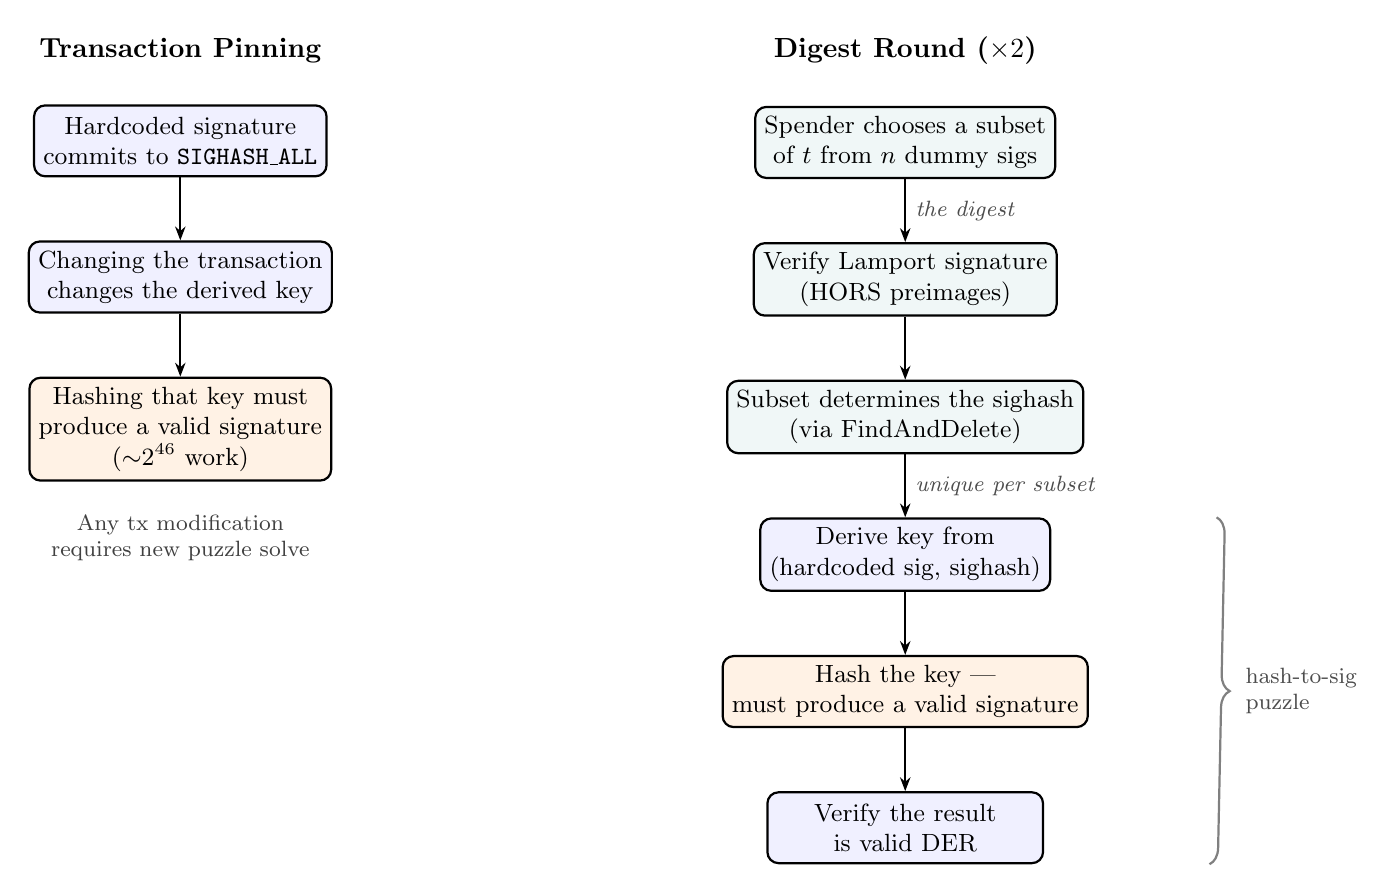
\begin{tikzpicture}[
    node distance=0.8cm and 1.2cm,
    every node/.style={font=\small},
    box/.style={draw, rounded corners=4pt, minimum height=0.9cm, minimum width=3.5cm, text centered, thick, align=center, fill=white},
    pin/.style={box, fill=blue!6},
    rnd/.style={box, fill=teal!6},
    hl/.style={box, fill=orange!10},
    arrow/.style={-{Stealth[length=5pt]}, thick},
]

% === PINNING ===
\node[font=\bfseries\normalsize] (pin_title) {Transaction Pinning};
\node[pin, below=0.4cm of pin_title] (p1) {Hardcoded signature\\commits to \texttt{SIGHASH\_ALL}};
\node[pin, below=of p1] (p2) {Changing the transaction\\changes the derived key};
\node[hl, below=of p2] (p3) {Hashing that key must\\produce a valid signature\\(${\sim}2^{46}$ work)};

\draw[arrow] (p1) -- (p2);
\draw[arrow] (p2) -- (p3);

\node[below=0.3cm of p3, font=\footnotesize, text=gray!50!black, align=center] {Any tx modification\\requires new puzzle solve};

% === ROUND (single, representative) ===
\node[font=\bfseries\normalsize, right=5.5cm of pin_title] (r_title) {Digest Round ($\times 2$)};

\node[rnd, below=0.4cm of r_title] (r1) {Spender chooses a subset\\of $t$ from $n$ dummy sigs};
\node[rnd, below=of r1] (r2) {Verify Lamport signature\\(HORS preimages)};
\node[rnd, below=of r2] (r3) {Subset determines the sighash\\(via FindAndDelete)};
\node[pin, below=of r3] (r4) {Derive key from\\(hardcoded sig, sighash)};
\node[hl, below=of r4] (r5) {Hash the key ---\\must produce a valid signature};
\node[pin, below=of r5] (r6) {Verify the result\\is valid DER};

\draw[arrow] (r1) -- node[right, font=\footnotesize\itshape, text=gray!60!black] {the digest} (r2);
\draw[arrow] (r2) -- (r3);
\draw[arrow] (r3) -- node[right, font=\footnotesize\itshape, text=gray!60!black] {unique per subset} (r4);
\draw[arrow] (r4) -- (r5);
\draw[arrow] (r5) -- (r6);

% Brace on right side
\draw[decorate, decoration={brace, amplitude=6pt}, thick, gray]
    ([xshift=2.1cm]r4.north east) -- ([xshift=2.1cm]r6.south east)
    node[midway, right=8pt, font=\footnotesize, text=gray!60!black, align=left] {hash-to-sig\\puzzle};

\end{tikzpicture}
\caption{The quantum-safe \textsc{Binohash} scheme. \textbf{Left:} transaction pinning ensures each transaction attempt costs ${\sim}2^{46}$ work. \textbf{Right:} each digest round selects a subset (the digest), verifies its Lamport signature, then checks the hash-to-sig puzzle---the subset that produces a valid RIPEMD-160 output is the solution. Two independent rounds are executed.}
\label{fig:qs-scheme}
\end{figure}

\paragraph{Bonus Keys.}
An optimization that reduces off-chain cost by adding extra selections that participate in FindAndDelete but skip HORS verification. Bonus keys cost only 3 opcodes per selection (vs.\ 9 for signed), and increase the effective subset count to match the~$2^{46}$ puzzle target. We analyze bonus keys and their security implications in Section~\ref{sec:bonus-keys}.

\subsection{Spending Procedure (Off-Chain)}
\label{sec:spending-procedure}

To spend a QSB-protected UTXO, the spender performs the following off-chain procedure:

\begin{enumerate}
    \item \textbf{Construct the transaction.} Set up the desired inputs, outputs, and other transaction fields.

    \item \textbf{Solve the pinning puzzle.} Vary any free transaction parameter that is committed to by \texttt{SIGHASH\_ALL}---such as \texttt{nLocktime}, \texttt{nSequence}, output amounts, change address, or \texttt{OP\_RETURN} data in an extra output---until~$\text{RIPEMD-160}(\mathit{key}_{\mathrm{nonce}})$ is a valid DER signature, where~$\mathit{key}_{\mathrm{nonce}}$ is derived via ECDSA key recovery from the hardcoded~$\mathit{sig}_{\mathrm{nonce}}$ and the current sighash. Any parameter that changes the sighash is equally valid; the choice is an implementation detail (see~\cite[Section~5.2]{linus2024binohash} for a discussion). This requires~${\sim}2^{46}$ attempts. The transaction is now fixed.

    \item \textbf{Search for the digest (per round).} Iterate over all~$\binom{n}{t}$ dummy signature subsets. For each subset, FindAndDelete produces a different scriptCode and therefore a different sighash. Recover~$\mathit{key}_{\mathrm{nonce}}$ from~$(\mathit{sig}_{\mathrm{nonce}}, \text{sighash})$ and compute~$\text{RIPEMD-160}(\mathit{key}_{\mathrm{nonce}})$. If the output is a valid DER signature, this subset is the digest for the round.

    \item \textbf{Repeat for both rounds.} If both rounds find a valid subset, the full digest is determined. Reveal the corresponding HORS preimages (Lamport signature) in the witness. If either round fails---none of the~$\binom{n}{t}$ subsets produces a valid DER output---return to step~1 with a different transaction and try again.
\end{enumerate}

\subsection{Operational Architecture}
\label{sec:operational-architecture}

A key operational advantage of QSB is the clean separation between the computationally intensive puzzle search and the security-sensitive signing operations. The search involves only public computations---ECDSA key recovery, RIPEMD-160 hashing, and sighash evaluation---none of which require private keys or secret data. This allows the search to be safely outsourced to untrusted hardware (e.g., rented GPU clusters), while all secrets remain on the spender's personal device.

\begin{figure}[H]
\centering
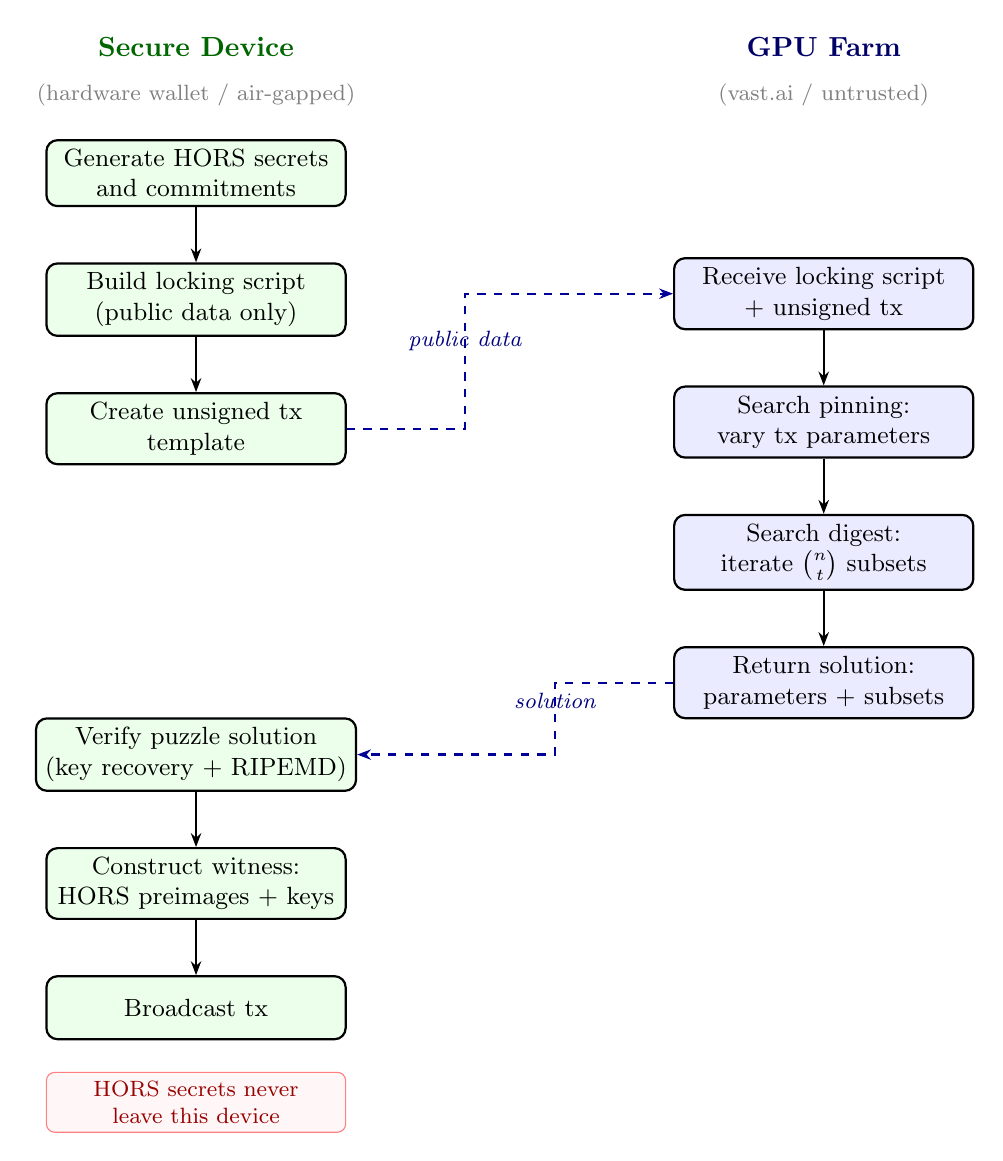
\begin{tikzpicture}[
    node distance=0.7cm and 3cm,
    every node/.style={font=\small},
    box/.style={draw, rounded corners=4pt, minimum height=0.8cm, minimum width=3.8cm, text centered, thick, align=center, fill=white},
    secure/.style={box, fill=green!8},
    gpu/.style={box, fill=blue!8},
    data/.style={-{Stealth[length=5pt]}, thick, dashed, blue!60!black},
    arrow/.style={-{Stealth[length=5pt]}, thick},
]

% === LEFT: Secure Device ===
\node[font=\bfseries\normalsize, text=green!40!black] (stitle) {Secure Device};
\node[font=\footnotesize, text=gray, below=0.1cm of stitle] (ssub) {(hardware wallet / air-gapped)};

\node[secure, below=0.3cm of ssub] (s1) {Generate HORS secrets\\and commitments};
\node[secure, below=of s1] (s2) {Build locking script\\(public data only)};
\node[secure, below=of s2] (s3) {Create unsigned tx\\template};
\node[secure, below=3.2cm of s3] (s4) {Verify puzzle solution\\(key recovery + RIPEMD)};
\node[secure, below=of s4] (s5) {Construct witness:\\HORS preimages + keys};
\node[secure, below=of s5] (s6) {Broadcast tx};

\draw[arrow] (s1) -- (s2);
\draw[arrow] (s2) -- (s3);
\draw[arrow] (s4) -- (s5);
\draw[arrow] (s5) -- (s6);

% === RIGHT: GPU Farm ===
\node[font=\bfseries\normalsize, text=blue!40!black, right=5.5cm of stitle] (gtitle) {GPU Farm};
\node[font=\footnotesize, text=gray, below=0.1cm of gtitle] (gsub) {(vast.ai / untrusted)};

\node[gpu, below=1.8cm of gsub] (g1) {Receive locking script\\+ unsigned tx};
\node[gpu, below=of g1] (g2) {Search pinning:\\vary tx parameters};
\node[gpu, below=of g2] (g3) {Search digest:\\iterate $\binom{n}{t}$ subsets};
\node[gpu, below=of g3] (g4) {Return solution:\\parameters + subsets};

\draw[arrow] (g1) -- (g2);
\draw[arrow] (g2) -- (g3);
\draw[arrow] (g3) -- (g4);

% === Data flow between them ===
\draw[data] (s3.east) -- +(1.5,0) |- (g1.west) node[pos=0.25, above, font=\footnotesize\itshape, text=blue!50!black] {public data};
\draw[data] (g4.west) -- +(-1.5,0) |- (s4.east) node[pos=0.25, above, font=\footnotesize\itshape, text=blue!50!black] {solution};

% === Annotation ===
\node[draw=red!50, rounded corners=3pt, fill=red!3, font=\footnotesize, text=red!60!black, align=center, below=0.4cm of s6, minimum width=3.8cm] (note) {HORS secrets never\\leave this device};

\end{tikzpicture}
\caption{Operational architecture. The GPU farm performs only public computations (key recovery, hashing). All secrets---HORS preimages---remain on the secure device. The spender verifies the solution locally before constructing the witness and broadcasting.}
\label{fig:operational-architecture}
\end{figure}

\paragraph{What the GPU farm receives.}
The locking script (containing HORS commitments, dummy signatures, and hardcoded~$\mathit{sig}_{\mathrm{nonce}}$ values) and an unsigned transaction template. All of this is public data.

\paragraph{What the GPU farm computes.}
For each candidate (transaction parameter variant or subset): compute the sighash, recover~$\mathit{key}_{\mathrm{nonce}}$ via ECDSA key recovery, compute RIPEMD-160, and check DER validity. These are all public operations---no private key or secret is involved.

\paragraph{What the GPU farm returns.}
The winning transaction parameters and subset indices. The spender's device independently verifies the solution (a single key recovery + RIPEMD-160 per round), then constructs the full witness by revealing the HORS preimages for the winning subsets.

\paragraph{Polyglot digest optimization.}
\textsc{Binohash}~\cite[Appendix~D]{linus2024binohash} proposes a ``polyglot digest'' optimization that merges dummy signatures and HORS commitments into a single element: grind a preimage~$P_i$ such that $\text{RIPEMD-160}(P_i)$ is a valid DER signature. Then~$P_i$ serves as the HORS preimage, while its hash serves as the dummy signature. This eliminates the need for separate dummy signature pushes, saving~${\sim}10$ bytes and 2 opcodes per selection---enabling higher~$t$ values (e.g., $t = 10$) or smaller~$n$ within the same budget. The paper acknowledges two costs: (1)~a one-time off-chain grinding cost of~${\sim}2^{53.5}$ RIPEMD-160 hashes to prepare the polyglot elements (pure hashing, no sighash computation), and (2)~the polyglot preimages are HORS secrets, so the grinding must be performed on trusted hardware. In our operational architecture, we require that all secrets remain on the spender's secure device. If the polyglot grinding exceeds that device's capacity and must be outsourced to a GPU farm, the farm would learn the HORS signing keys. We therefore do not adopt this optimization, though it remains a promising direction if the trusted-hardware constraint can be relaxed.

\paragraph{Transaction broadcast.}
QSB transactions are consensus-valid but non-standard: bare scripts exceeding the default relay policy limits are not propagated by standard Bitcoin Core nodes. As with \textsc{Binohash}~\cite[Section~6]{linus2024binohash}, broadcasting requires submitting the transaction directly to a mining pool that accepts non-standard transactions, such as via a private mempool service (e.g., Marathon's Slipstream).

% ============================================================
\section{Security and Cost Analysis}
\label{sec:security-cost}
% ============================================================

We analyze the security of our scheme for the baseline configuration: $n = 150$, $t = 8$ signed selections per round, two rounds. The puzzle target is fixed at~${\sim}2^{46}$ (RIPEMD-160).

\subsection{Baseline: $t = 8$, $t = 8$}
\label{sec:baseline}

\begin{center}
\begin{tabular}{ll}
\toprule
\textbf{Property} & \textbf{Value} \\
\midrule
Non-push opcodes & 197 / 201 (4 spare) \\
Script size & ${\sim}9{,}650$ / 10{,}000 bytes \\
\midrule
Subsets per round & $\binom{150}{8} \approx 2^{42.3}$ \\
Puzzle target per round & ${\sim}2^{46}$ (RIPEMD-160) \\
Digest size & $2 \times 42.3 = 84.5$ bits \\
\midrule
Tx grinds & $\left(2^{46} / 2^{42.3}\right)^2 \approx 2^{7.5}$ (${\approx}180$ attempts) \\
Honest spender work & ${\sim}2^{53.5}$ \\
\midrule
Second pre-image resistance & ${\sim}2^{138}$ \\
Collision resistance & ${\sim}2^{88}$ \\
\bottomrule
\end{tabular}
\end{center}

\subsection{Opcode and Script Size Budget}
\label{sec:budget}

\paragraph{Opcodes.}
The pinning stage costs 5 non-push opcodes. Each digest round costs:
$$11 t + 8$$
where $t$ is the number of \emph{signed} selections per round (with no bonus keys). The breakdown is: $9t$ for the selection loop (9 opcodes per selection) and $2t + 8$ for the puzzle derivation, \texttt{CHECKSIGVERIFY}, and \texttt{CHECKMULTISIG} setup. For two rounds with $t_1$ and $t_2$ signed selections, the total is:
$$5 + (11 t_1 + 8) + (11 t_2 + 8) = 11(t_1 + t_2) + 21 \leq 201$$

\noindent When bonus keys are used, the per-round formula generalizes to $9 t_{\mathrm{signed}} + 3 t_{\mathrm{bonus}} + 2 t_{\mathrm{total}} + 8$ (see Section~\ref{sec:bonus-keys}).

\paragraph{Script size.}
The pinning stage occupies approximately 15 bytes (a 9-byte signature push plus 5 opcode bytes). Each digest round occupies approximately:
$$31n + 13 t + 20 \text{ bytes}$$
The dominant term is~$31n$: each of the~$n$ pool entries contributes a 20-byte HORS commitment (plus 1-byte push opcode) and a 9-byte dummy signature (plus 1-byte push opcode). The remaining terms account for the selection logic, puzzle verification, and \texttt{CHECKMULTISIG} setup. For two rounds, the total is approximately~$62n + \text{overhead} \leq 10{,}000$.

At $n = 150$, each additional pool entry costs~${\sim}62$ bytes across both rounds, while adding~${\sim}0.08$ bits of digest entropy per entry.

\subsection{Security and Grinding Analysis}
\label{sec:security-detail}

\paragraph{Second pre-image resistance.}
An attacker who observes a valid spending transaction must find a different transaction that produces the same digest---the same signed indices in both rounds. Each transaction attempt costs~$2^{46}$ (the pinning puzzle). For each pinned transaction, the probability that a specific $t$-subset solves the round puzzle is~$2^{-46}$. Since both rounds must independently match, the probability per pinned attempt is~$2^{-92}$. The total cost is therefore~$2^{46} \times 2^{92} = 2^{138}$.

\paragraph{Collision resistance.}
A malicious spender who controls the transaction creation process aims to find two transactions with the same digest. The digest space is~$2^{84.5}$. By the birthday bound, ${\sim}2^{42.3}$ samples suffice to find a collision. Each sample costs~$2^{46}$ (pinning), giving a total collision cost of~$2^{46 + 42.3} \approx 2^{88}$.

\paragraph{Honest spender: subset mismatch.}
The subsets per round ($\binom{150}{8} \approx 2^{42.3}$) fall short of the~$2^{46}$ puzzle target by a factor of~$2^{3.7}$. This means each round has only a~$2^{-3.7}$ probability of containing a valid subset for a given pinned transaction. Since both rounds must succeed, the spender needs on average~${\sim}2^{7.5} \approx 180$ pinned transaction attempts. Each attempt requires iterating over all~$\binom{150}{8}$ subsets per round, giving a total work of~${\sim}2^{53.5}$ RIPEMD-160 evaluations. The actual wall-clock cost depends on implementation; we defer this estimate to Section~\ref{sec:offchain-cost}.

\subsection{Quantum Security}
\label{sec:quantum-security}

We analyze the security of the baseline configuration under quantum adversaries, distinguishing between two threat levels introduced in Section~\ref{sec:quantum-assumptions}.

\paragraph{Shor's algorithm only (ECDSA broken, hash functions unaffected).}
This is the primary threat our scheme is designed to resist. A quantum adversary running Shor's algorithm can compute discrete logarithms and forge ECDSA signatures, but cannot speed up hash function evaluation.

Under this model, the security of our scheme is \emph{identical} to the classical case:

\begin{center}
\begin{tabular}{lll}
\toprule
\textbf{Property} & \textbf{Classical} & \textbf{Shor only} \\
\midrule
Pinning cost & $2^{46}$ & $2^{46}$ (hash-based) \\
Second pre-image & $2^{138}$ & $2^{138}$ \\
Collision & $2^{88}$ & $2^{88}$ \\
\bottomrule
\end{tabular}
\end{center}

\noindent This is the central result: because our puzzle relies on RIPEMD-160 pre-image resistance rather than ECDSA hardness, Shor's algorithm provides \emph{no advantage} to the attacker. The scheme achieves full classical security even against a quantum adversary with unbounded access to Shor's algorithm.

\paragraph{Grover's algorithm (quadratic speedup on hash search).}
Grover's algorithm~\cite{grover1996} provides a quadratic speedup for unstructured search problems. Applied to our scheme, it reduces the effective security:

\begin{center}
\begin{tabular}{lll}
\toprule
\textbf{Property} & \textbf{Classical} & \textbf{With Grover} \\
\midrule
Pinning cost & $2^{46}$ & ${\sim}2^{23}$ \\
Second pre-image & $2^{138}$ & ${\sim}2^{69}$ \\
Collision & $2^{88}$ & ${\sim}2^{65}$ \\
\bottomrule
\end{tabular}
\end{center}

\noindent For second pre-image resistance, Grover provides a square-root speedup on the full search: the classical cost of~$2^{138}$ becomes~${\sim}2^{69}$. For collision resistance, the pinning cost per sample drops from~$2^{46}$ to~${\sim}2^{23}$, while the birthday bound remains at~$2^{42.3}$ samples, giving~$2^{23 + 42.3} \approx 2^{65}$.

\paragraph{Practical feasibility of Grover.}
While these reductions appear significant on paper, Grover's algorithm faces fundamental limitations that make it far less threatening than Shor's in practice. Grover cannot be efficiently parallelized: running~$k$ quantum computers in parallel provides only a~$\sqrt{k}$ speedup, not a~$k$-fold speedup~\cite{grover1996}. Moreover, implementing the search oracle as a quantum circuit requires all intermediate state---including the sighash computation (SHA-256d) and key recovery---to be represented in reversible logic, demanding significant qubit overhead.

More importantly, Shor's algorithm for the secp256k1 curve requires on the order of a few thousand logical qubits and is expected to be feasible well before Grover becomes practical against targets of~$2^{46}$ or higher. This asymmetry is precisely why eliminating reliance on ECDSA hardness---while retaining hash-based security---is the right design strategy. Note that with bonus keys (Section~\ref{sec:bonus-keys}), the recommended Config~A trades some security for reduced cost, achieving~$2^{118}$ pre-image and~$2^{78}$ collision resistance.

\subsection{Bonus Keys}
\label{sec:bonus-keys}

\paragraph{Motivation.}
The baseline configuration ($t = 8$, $t = 8$) achieves strong security but incurs significant off-chain cost. The problem is the \emph{subset mismatch}: each round offers $\binom{150}{8} \approx 2^{42.3}$ subsets, but the RIPEMD-160 puzzle target is fixed at~${\sim}2^{46}$. The gap of~$2^{3.7}$ means that for a given pinned transaction, each round has only a~$2^{-3.7} \approx 8\%$ chance of containing a valid subset. Since both rounds must succeed, the spender needs~${\sim}2^{7.5} \approx 180$ pinned transaction attempts, each requiring~$2^{46}$ work.

The ideal remedy is to increase the subset count to~$\binom{150}{t} \geq 2^{46}$. This requires $t \geq 9$, since $\binom{150}{9} \approx 2^{46.2}$. However, adding a fully signed selection costs 9 opcodes, and the opcode budget is already tight at 197 / 201.

\paragraph{The bonus key optimization.}
A \emph{bonus key} is a subset selection that participates in FindAndDelete---contributing to $\binom{n}{t_{\mathrm{total}}}$ and increasing the number of sighash candidates---but skips HORS verification. Because the HORS check (DUP + ADD + ROLL + ROLL + HASH160 + EQUALVERIFY) is omitted, a bonus selection costs only \textbf{3 opcodes} instead of 9:

\begin{lstlisting}[language={}, numbers=none]
// Bonus selection (3 ops):
{pos} OP_ROLL          // roll index from witness
{n-i} OP_MIN           // sanitize
OP_ROLL                // roll dummy sig
\end{lstlisting}

\noindent With $t_{\mathrm{signed}} = 8$ and $t_{\mathrm{bonus}} = 1$, the effective subset count becomes $\binom{150}{9} \approx 2^{46.2}$, which exceeds the puzzle target. The spender now finds a valid subset in almost every pinned transaction, eliminating the grinding overhead.

The per-round opcode formula generalizes to:
$$9 t_{\mathrm{signed}} + 3 t_{\mathrm{bonus}} + 2 t_{\mathrm{total}} + 8$$

\paragraph{Security impact.}
Bonus keys reduce security because they give the attacker additional freedom:

\begin{itemize}
    \item \textbf{Pre-image}: The attacker knows the signed indices (from revealed HORS preimages) but can freely choose bonus indices. For a round with $t_{\mathrm{signed}}$ signed and $t_{\mathrm{bonus}}$ bonus keys, the attacker gets $\binom{n - t_{\mathrm{signed}}}{t_{\mathrm{bonus}}}$ free bonus combinations per pinned transaction, each producing a different sighash. This reduces the pre-image cost by a factor of~$\binom{n - t_{\mathrm{signed}}}{t_{\mathrm{bonus}}}$ per round.

    \item \textbf{Collision}: The attacker can assign which of the $t_{\mathrm{total}}$ passing indices are ``signed'' versus ``bonus.'' This gives $\binom{t_{\mathrm{total}}}{t_{\mathrm{signed}}}$ digest choices per passing subset per round, effectively multiplying the birthday attack.
\end{itemize}

\paragraph{Configurations.}

\begin{center}
\small
\begin{tabular}{lcccccc}
\toprule
\textbf{Config} & \textbf{Ops} & \textbf{Digest} & \textbf{Pre-image} & \textbf{Collision} & \textbf{Grinds} \\
\midrule
$t{=}8, 8$ (baseline) & 197 (+4) & 84.5b & $2^{138}$ & $2^{88}$ & ${\sim}180\times$ \\
$t{=}8{+}1\mathrm{b}, 8$ & 202 ($-1$) & 84.5b & $2^{131}$ & $2^{85}$ & ${\sim}13\times$ \\
$t{=}8{+}1\mathrm{b}, 7{+}2\mathrm{b}$ & 201 (+0) & 80.4b & $2^{118}$ & $2^{78}$ & ${\sim}1\times$ \\
\bottomrule
\end{tabular}
\end{center}

\noindent Config~A ($t = 8{+}1\mathrm{b}, 7{+}2\mathrm{b}$) fits exactly within the 201-opcode limit and eliminates grinding entirely ($\binom{150}{9} \approx 2^{46.2} \geq 2^{46}$ in both rounds). The security penalty is~${\sim}8$ bits on both pre-image and collision resistance. Config~B ($t = 8{+}1\mathrm{b}, 8$) preserves full digest entropy but exceeds the opcode limit by~1.

\subsection{Off-Chain Cost}
\label{sec:offchain-cost}

The off-chain cost of spending a QSB transaction is dominated by the search for valid subsets across both digest rounds. We estimate costs relative to \textsc{Binohash}, which reports a cost of~${\sim}\$50$ in GPU compute~\cite{linus2024binohash}.

\paragraph{Cost structure.}
For each candidate subset, the spender must:
\begin{enumerate}
    \item Apply FindAndDelete to remove the selected dummy signatures from the scriptCode.
    \item Compute the sighash (SHA-256d of the~${\sim}5$\,KB modified scriptCode).
    \item Recover the public key via ECDSA key recovery.
    \item Compute RIPEMD-160 of the recovered key and check for valid DER.
\end{enumerate}

Steps~1--2 (sighash computation) dominate the per-candidate cost and are shared with \textsc{Binohash}. Step~3 (EC recovery, ${\sim}10\,\mu$s on CPU) adds overhead that \textsc{Binohash} avoids, since its OP\_SIZE puzzle requires only an ECDSA sign (${\sim}1\,\mu$s).

\paragraph{Incremental sighash optimization.}
The sighash cost can be reduced by precomputing SHA-256 states over the fixed portions of the scriptCode. The HORS commitments (${\sim}3{,}150$ bytes) are identical across all subsets and can be precomputed once. Furthermore, when searching Round~2, the entire Round~1 section (${\sim}4{,}850$ bytes) is unaffected by FindAndDelete and forms a fixed prefix, allowing precomputation of~${\sim}125$ out of~${\sim}152$ SHA-256 blocks. For pinning, only a few bytes change per candidate (e.g., \texttt{nLocktime} or \texttt{nSequence}), allowing precomputation of all but the final SHA-256 block.

\begin{center}
\small
\begin{tabular}{lccc}
\toprule
\textbf{Phase} & \textbf{SHA blocks/candidate} & \textbf{EC cost} & \textbf{Total} \\
\midrule
Pinning & 1 (of 152) & ${\sim}10\,\mu$s & ${\sim}10\,\mu$s \\
Round 1 & ${\sim}102$ (of 152) & ${\sim}10\,\mu$s & ${\sim}41\,\mu$s \\
Round 2 & ${\sim}27$ (of 152) & ${\sim}10\,\mu$s & ${\sim}18\,\mu$s \\
\bottomrule
\end{tabular}
\end{center}

\paragraph{Comparison with Binohash.}
QSB is more expensive than \textsc{Binohash} for two reasons:

\begin{enumerate}
    \item \textbf{Larger search space.} The RIPEMD-160 puzzle target ($2^{46}$) is fixed and cannot be tuned to match $\binom{n}{t}$. With Config~A ($t_{\mathrm{total}} = 9$), $\binom{150}{9} \approx 2^{46.2}$ closely matches the target, but \textsc{Binohash} can tune its OP\_SIZE target to exactly match $\binom{150}{8} \approx 2^{42.3}$. This results in ${\sim}16\times$ more subsets to search per round.

    \item \textbf{EC recovery overhead.} Each QSB candidate requires ECDSA key recovery (${\sim}10\,\mu$s) rather than ECDSA signing (${\sim}1\,\mu$s). However, since the sighash computation (${\sim}8$--$30\,\mu$s per candidate with precomputation) dominates, the per-candidate overhead is only~${\sim}1.3\times$.
\end{enumerate}

\noindent The combined overhead depends on the optimization level. At the raw work level, QSB requires~$2^{47.7}$ total candidates versus \textsc{Binohash}'s~$2^{44.6}$---a ratio of~${\sim}9\times$. The per-candidate cost ratio varies from~$0.5\times$ (if QSB applies incremental sighash but \textsc{Binohash} does not) to~${\sim}2.5\times$ (if both are fully optimized and EC recovery dominates), depending on implementation.

Calibrating against \textsc{Binohash}'s reported~${\sim}\$50$ GPU cost for~$2^{44.6}$ honest work~\cite{linus2024binohash}, we estimate:

\begin{center}
\begin{tabular}{lcc}
\toprule
\textbf{Scheme} & \textbf{Honest work} & \textbf{GPU cost} \\
\midrule
\textsc{Binohash} ($t{=}8, 8$, $W_1{=}W_2{=}42$) & $2^{44.6}$ & ${\sim}\$50$ \\
QSB Config~A ($t{=}8{+}1\mathrm{b}, 7{+}2\mathrm{b}$) & $2^{47.7}$ & ${\sim}\$75$--$\$200$ \\
\bottomrule
\end{tabular}
\end{center}

\noindent The range reflects uncertainty about the relative optimization levels. The fundamental overhead is~${\sim}9\times$ in raw work, driven primarily by the larger subset space ($\binom{150}{9}$ vs.~$\binom{150}{8}$ per round). This is the cost of quantum safety under Shor's algorithm.

\paragraph{Measured cost breakdown.}
Using a GPU implementation with SHA-256 midstate precomputation and precomputed EC lookup tables, the off-chain computation consists of three phases: transaction pinning (${\sim}\$25$--$\$50$), and two rounds of digest search (${\sim}\$25$--$\$50$ each), for a total of ${\sim}\$75$--$\$150$ on commodity cloud GPUs at current spot pricing. The computation is embarrassingly parallel, so wall-clock time scales inversely with the number of GPUs.

% ============================================================
\section{Conclusion}
\label{sec:conclusion}
% ============================================================

We have presented Quantum Safe Bitcoin (QSB), a modification of \textsc{Binohash}~\cite{linus2024binohash} that eliminates the scheme's reliance on Shor-breakable assumptions. The key change is replacing the signature-size puzzle---which depends on the hardness of finding small elliptic curve $r$-coordinates---with a hash-to-sig puzzle whose security rests entirely on the pre-image resistance of RIPEMD-160. This enables signing Bitcoin transactions in a quantum-safe manner today, without any changes to the Bitcoin protocol: QSB operates under the existing consensus rules for legacy transactions. To the best of our knowledge, this is the first scheme to achieve quantum-safe Bitcoin transactions on the live network.

The scheme offers a tunable tradeoff between security and off-chain cost. Using bonus keys, the spender can match the subset count to the fixed $2^{46}$ puzzle target, eliminating grinding overhead at the cost of a modest reduction in digest entropy. The resulting configuration (Config~A) achieves ${\sim}118$-bit pre-image resistance and ${\sim}78$-bit collision resistance, with an estimated off-chain GPU cost on the order of a few hundred dollars---roughly $5$--$10\times$ that of \textsc{Binohash}.

Our main contributions are:

\begin{enumerate}
    \item \textbf{Hash-to-signature puzzle.} Replacing the OP\_SIZE-based signature puzzle with a RIPEMD-160 hash-to-sig puzzle, achieving quantum safety. As a side effect, the hardcoded \texttt{SIGHASH\_ALL} flag in our puzzle resolves the sighash flag uncertainty identified in \textsc{Binohash}.

    \item \textbf{Bonus keys.} Introducing bonus selections that participate in FindAndDelete without HORS verification, providing a flexible tradeoff between security and off-chain cost within the tight 201-opcode budget.
\end{enumerate}

\subsection{Future Work}

\begin{itemize}
    \item Improved opcode utilization to increase security margins.
    \item Formal security proofs of the protocol.
    \item Exploration of other applications of QSB beyond quantum safety---such as a more widely used tool for transaction introspection, as it resolves the sighash flag uncertainty present in \textsc{Binohash}.
\end{itemize}

\subsection*{Acknowledgements}

We thank Robin Linus for useful discussions about \textsc{Binohash}. We also thank Eli Ben-Sasson and Adam Borco for comments that helped improve the presentation of this article.

\begin{thebibliography}{9}
\bibitem{heilman2024}
    E.~Heilman,
    ``Signing a Bitcoin Transaction with Lamport Signatures (no OP\_CAT),''
    Bitcoin Development Mailing List, 2024.
    \url{https://groups.google.com/g/bitcoindev/c/mR53go5gHIk}

\bibitem{linus2024binohash}
    R.~Linus,
    ``Binohash: Transaction Introspection Without Softforks,''
    2026.
    \url{https://robinlinus.com/binohash.pdf}

\bibitem{bip341}
    P.~Wuille, J.~Nick, and T.~Ruffing,
    ``BIP 341: Taproot: SegWit version 1 spending rules,''
    Bitcoin Improvement Proposals, 2020.
    \url{https://github.com/bitcoin/bips/blob/master/bip-0341.mediawiki}

\bibitem{borco2024}
    A.~Bor,
    ``BTC PoW Locked Outputs,''
    GitHub, 2024.
    \url{https://github.com/adambor/btc-pow-locked-outputs}

\bibitem{bip143}
    J.~Lau and E.~Lombrozo,
    ``BIP 143: Transaction Signature Verification for Version 0 Witness Program,''
    Bitcoin Improvement Proposals, 2016.
    \url{https://github.com/bitcoin/bips/blob/master/bip-0143.mediawiki}

\bibitem{shor1994}
    P.~W.~Shor,
    ``Algorithms for Quantum Computation: Discrete Logarithms and Factoring,''
    Proceedings of the 35th Annual Symposium on Foundations of Computer Science, pp.~124--134, 1994.

\bibitem{grover1996}
    L.~K.~Grover,
    ``A Fast Quantum Mechanical Algorithm for Database Search,''
    Proceedings of the 28th Annual ACM Symposium on Theory of Computing, pp.~212--219, 1996.

\bibitem{linus2024sha2ecdsa}
    R.~Linus,
    ``SHA-2 ECDSA,''
    GitHub, 2024.
    \url{https://github.com/RobinLinus/sha2-ecdsa}

\bibitem{reyzin2002}
    L.~Reyzin and N.~Reyzin,
    ``Better than BiBa: Short One-Time Signatures with Fast Signing and Verifying,''
    Proceedings of ACISP, pp.~144--153, 2002.
\end{thebibliography}

\appendix

\section{Subset Selection Script}
\label{app:selection-script}

The following script implements a single signed selection iteration (Stage~1 of a digest round, Section~\ref{sec:qs-rounds}). It is repeated~$t_{\mathrm{signed}}$ times, with the position constants adjusted for each iteration~$i$:

\begin{lstlisting}[language={}, numbers=none]
// Signed selection i (9 opcodes):
{2n+1-i} OP_ROLL           // roll index from witness
{n-i} OP_MIN                // sanitize (prevent out-of-bounds)
OP_DUP                      // copy index (needed for sig lookup)
{n+1} OP_ADD                // compute commitment position
OP_ROLL                     // roll HORS commitment to top
{2n+1+t-2i} OP_ROLL         // roll HORS preimage from witness
OP_HASH160                  // hash preimage
OP_EQUALVERIFY              // verify preimage matches commitment
OP_ROLL                     // roll dummy sig (using index on stack)
\end{lstlisting}

\noindent This is identical to the selection loop in \textsc{Binohash}~\cite[Appendix~B]{linus2024binohash}. The position constants account for~$\mathit{sig}_{\mathrm{nonce}}$ being on the stack above the dummy signatures (hence $2n + 1$ rather than $2n$).

\section{Full QSB Script ($t = 8$, $t = 8$, $n = 150$)}
\label{app:full-script}

The complete locking script for the baseline configuration (197 opcodes, ${\sim}9{,}650$ bytes). HORS commitments and dummy signatures are abbreviated.

\begin{lstlisting}[language={}, numbers=none]
// ============================================================
// PINNING (5 opcodes)
// ============================================================
// Witness: <key_puzzle> <key_nonce>

<sig_nonce>                     // 9 bytes, hardcoded, SIGHASH_ALL
OP_OVER                         // [1] copy key_nonce
OP_CHECKSIGVERIFY               // [2] verify (sig_nonce, key_nonce)
OP_RIPEMD160                    // [3] key_nonce -> sig_puzzle
OP_SWAP                         // [4] get key_puzzle on top
OP_CHECKSIGVERIFY               // [5] verify (sig_puzzle, key_puzzle)


// ============================================================
// ROUND 1 (96 opcodes)
// ============================================================

// --- 150 HORS commitments (20 bytes each) ---
<H(pre_149)_r1>
<H(pre_148)_r1>
...
<H(pre_000)_r1>

// --- 150 dummy sigs (9 bytes each, SIGHASH_SINGLE) ---
<sig_149_r1>
<sig_148_r1>
...
<sig_000_r1>

OP_0                            // CHECKMULTISIG dummy
<sig_nonce_r1>                  // 9 bytes, hardcoded, SIGHASH_ALL

// --- 8 signed selections (9 ops each = 72 ops) ---
// Selection 0:
301 OP_ROLL                     // roll index_0 from witness
150 OP_MIN                      // sanitize
OP_DUP                          // copy index
151 OP_ADD                      // commitment position
OP_ROLL                         // roll commitment
309 OP_ROLL                     // roll preimage_0 from witness
OP_HASH160                      // hash preimage
OP_EQUALVERIFY                  // verify HORS
OP_ROLL                         // roll dummy sig
// Selections 1--7: (same structure, adjusted positions)
...

// --- Puzzle + CHECKMULTISIG (24 ops) ---
302 OP_ROLL                     // roll key_nonce from witness
OP_DUP                          // copy for RIPEMD + pubkey
OP_RIPEMD160                    // key_nonce -> sig_puzzle

302 OP_ROLL                     // roll key_puzzle from witness
OP_CHECKSIGVERIFY               // verify (sig_puzzle, key_puzzle)

OP_9                            // M = 9 (8 dummies + sig_nonce)
OP_2 OP_ROLL                    // move key_nonce into pubkey zone
302 OP_ROLL                     // roll pub_0
...                             // (8 rolls total)
302 OP_ROLL                     // roll pub_7
OP_9                            // N = 9
OP_CHECKMULTISIG                // verify all 9 sig/key pairs


// ============================================================
// ROUND 2 (96 opcodes) -- same structure as Round 1
// ============================================================
// (identical structure, independent data)
...
\end{lstlisting}

\noindent Full annotated scripts with exact position constants for multiple configurations are available at: \url{https://github.com/avihu28/quantum-safe-bitcoin-tx}

\end{document}
